\documentclass{article}

\usepackage{amsmath}
\usepackage{graphicx}
\usepackage{titlesec}
\usepackage[hidelinks]{hyperref}
\usepackage[backend=biber,natbib=true]{biblatex}
\addbibresource{Interpolations.bib}

\setcounter{secnumdepth}{4}
\setcounter{tocdepth}{4}
\titleformat{\paragraph}
{\normalfont\normalsize\bfseries}{\theparagraph}{1em}{}
\titlespacing*{\paragraph}
{0pt}{3.25ex plus 1ex minus .2ex}{1.5ex plus .2ex}


\author{Tomas Lycken\\tomas.lycken@gmail.com\\github.com/tlycken}
\title{\texttt{Interpolations.jl} - mathematical background}

\begin{document}

\maketitle
\abstract{This document intends to outline the mathematical foundations of the \texttt{Interpolations.jl} package, in order to make it easier to understand how the library works, as well as to change or extend its behavior. Since it shows off the derivations that underlie the code, it is also intended to help figuring out if a bug stems from coding or mathematical mistakes.}

\newpage
\tableofcontents
\newpage

\section{Introduction}
Interpolations.jl uses \emph{B-splines}\footnote{\url{http://en.wikipedia.org/wiki/B-spline\#Definition}}, or \emph{basis splines}, to interpolate a data set with a specified degree. In short, the idea is to use a set of basis functions with limited support, and in each interval between two data points, construct a linear combination of the basis functions which have support in that interval, each yielding a piece in a piecewise defined function with support across the entire data set. B-splines are defined to have the maximum degree of continuity, with minimal support. Specific details on the general mathematics of such interpolations have been extensively presented by \citet{875199}.

Before going into specific implementation details, we must define a few core concepts.

\subsection{Interpolation degree}

The interpolation degree decides what continuity properties the interpolant (i.e. the object which represents the interpolated data set) has; for example, a linear interpolation is a piecewise linear function, which is continuous but has discontinuous derivatives (or gradients, in higher dimensions).

Because of how B-splines are defined, the interpolation degree also decides the \emph{support} of the \emph{spline functions}. For a linear interpolation, the function value is decided by the value at \emph{two} data points, so its support is two\footnote{For this reason, linear B-splines are often referred to as \emph{2nd order}, which may be a source of confusion since the interpolating function itself is linear, i.e. of first order. In \texttt{Interpolations.jl}, we will try to avoid this confusion by referring to interpolation degree by ``linear'', ``quadratic'' etc.}.


\subsection{Grid cells}

When looking at a discrete grid, one can consider the data points to define either cell boundaries (with one grid cell spanning the domain between two data points) or cell centers (with one grid cell spanning the domain closest to a single data point). On uniform, 1-spaced grids, this corresponds to having cell boundaries either at integers $1, 2, \ldots$ (where the data points are specified), or at half-integers $\frac{1}{2}, \frac{3}{2}, \ldots$ (exactly centered between data points).

Each interpolation type defines a \emph{grid behavior}, specified by \texttt{OnGrid} or \texttt{OnCell}. However, interpolations of even (odd) degree will use an odd (even) number of points, and we require them to be symmetric. Thus, even (odd) degree interpolations will use \texttt{OnCell} (\texttt{OnGrid}) behavior inside the domain, regardless of the \texttt{OnCell} or \texttt{OnGrid} specification in the interpolation type; \texttt{OnCell}/\texttt{OnGrid} will be used solely to determine where the edges of the domain lie.

\subsection{Boundary conditions}

For higher interpolation degrees (specifically, from quadratic interpolation and up), the support of the B-splines is too large for the interpolating scheme to be able to figure out the values near the edges of the data sets. In order to close the equation systems at the edges, boundary conditions are used.

\subsection{Extrapolation behavior}

Somewhat orthogonal\footnote{Although the implementational separation of extrapolation behavior is computationally sound, it does allow for some interesting, yet probably nonsensical, combinations of interpolation degrees, boundary conditions and extrapolation behavior. In cases where the extrapolation behavior is defined as constant or reflecting, it will make sense to specify matching boundary conditions, but other combinations are entirely supported by \texttt{Interpolations.jl}. No guarantees are left that the results make sense, though...} to the concepts outlined above, is the concept of \emph{extrapolation}, i.e. evaluation of the interpolant outside the domain defined by the data set. For some types of extrapolation, this behavior is defined by a translation of the interpolation coordinate to somewhere inside the domain (e.g. periodic or reflecting boundaries), while for other types it entails a separate calculation entirely (e.g. linear extrapolation).

\section{Constant B-splines}

A constant ``polynomial'' has the form $p(x) = k$ for some constant $k$, and so requires only one parameter. A constant B-spline, therefore, has support 1. The intuitive way of understanding a constant B-spline is as a \emph{nearest neighbor} interpolation.

Constant B-splines are \emph{interpolating}, using the terminology of \citet{875199}, so there is no need to set up and solve an equation system for the interpolation coefficients; \texttt{Interpolations.jl} simply returns \texttt{A[round(Int,x)]} for constant interpolation of the vector \texttt{A}\footnote{Mathematically, there are a few different ways that points that are exactly between two data points are treated, depending on the source; in the case of \texttt{Interpolations.jl}, since we are dealing with floating point operations anyway, we use the result of \texttt{round(Int, x)} as the nearest neighbor index without worrying about the details.}.

\section{Linear B-splines}

Linear functions require two coefficients - the slope and the elevation; thus, linear B-splines have support 2. Linear B-splines are interpolating just like constant B-splines, so the data points can be used as interpolation coefficients without any pre-filtering. Linear B-splines are implemented in \texttt{Interpolations.jl} simply as a piecewise linear interpolation between the two nearest data points.

When \texttt{OnCell} behavior is specified, the outermost linear pieces are extended by a half-cell, effectively using linear extrapolation based on the two outermost data points, up to $\frac{1}{2}$ outside the provided data.

\section{Quadratic B-splines}

\subsection{Cell definition}
A quadratic polynomial requires three coefficients, and thus quadratic B-splines are \emph{three-point}, i.e. the interpolating spline function in one grid cell takes three provided data points into account. It is natural to center the grid cells around the middle point, so that the spline function around $x_i$ is is defined on the interval $\delta x \in [-\frac{1}{2}, \frac{1}{2}]$, where $\delta x = x - x_i$ and $i$ ranges from $1$ to the number of data points $N$.

\subsection{General governing equations}

Assuming a symmetric spline basis, one finds that 
\begin{align}
\label{bspline-quadratic-yi}
y_i(\delta x) &= c_{i-1}\left(\tfrac{1}{2} - \delta x\right)^{2} + c_{i}\left(\tfrac{3}{4} - \delta x^{2}\right) + c_{i+1}\left(\tfrac{1}{2} + \delta x\right)^{2}
\end{align}
Furthermore, we require that on cell boundaries, the function values and first derivatives are continuous, which yields $y_{i}(\frac{1}{2}) = y_{i+1}(-\frac{1}{2})$ and $y'_{i}(\frac{1}{2}) = y'_{i+1}(-\frac{1}{2})$. Inserting these in each-other, we find the following equation for each data point:
\begin{align*}\frac{1}{8} c_{i-1} + \frac{3}{4} c_{i} + \frac{1}{8} c_{i+1} = v_i\end{align*}
where $v_{i}$ is the provided data point at $x_{i}$. Considering the corresponding equation for all provided data points simultanesously, we form a tridiagonal equation system that we need to solve for the coefficients $c_{i}$. However, since we have two more unknowns than we have data points (namely $c_{0}$ and $c_{N+1}$), we need to apply boundary conditions to close the system.

\subsection{Boundary conditions}

The boundary conditions are implemented by specifying further conditions on the function value and/or its derivatives at the outer boundary (or, in some cases, close to it). For simplicity, we will here only describe the lower boundary close to $x = 1$, yielding equations for $c_0$ - the same arguments are applied at the upper end of the interval, specifying $c_{N+1}$.

We will have use for the following expressions for the first and second derivatives of the interpolating function:
\begin{align*}
y'_i(\delta x) &= \frac{1}{2}\left[c_{i-1}(2\delta x-1) - c_i \cdot 4\delta x + c_ {i+1} (2\delta x + 1)\right] \\
y''_i(\delta x) &= c_{i-1} - 2c_i + c_{i+1}
\end{align*}
which were obtained simply by derivation of equation \eqref{bspline-quadratic-yi} with respect to $\delta x$.

\subsubsection{Flat boundary conditions}

\texttt{Flat} boundary conditions are implemented by imposing that $y' = 0$ at the outermost cell boundary.

\paragraph{\texttt{Quadratic\{Flat,OnGrid\}}}
In this case, the edge is at $x=1$, corresponding to $(i,\delta x) = (1,0)$. Inserting this in $y'=0$ yields
\begin{align*}
y'(x_{\text{edge}}) = y'_1(0) &= \frac{1}{2}\left[-c_0 + c_2\right] = 0\\
\Rightarrow - c_0 + c_2 &= 0
\end{align*}
Thus, the first few rows of the equation system become
\begin{align*}
\begin{bmatrix} 
-1 & 0 & 1 \\
\frac{1}{8} & \frac{3}{4} & \frac{1}{8} \\
 & \frac{1}{8} & \frac{3}{4} & \frac{1}{8} \\
 & & \ddots & \ddots & \ddots
\end{bmatrix}
\begin{bmatrix}c_0\\ c_1\\ c_2\\\vdots\end{bmatrix}
&=
\begin{bmatrix}0\\ v_1 \\ v_2 \\\vdots\end{bmatrix}
\end{align*}

\paragraph{\texttt{Quadratic\{Flat,OnCell\}}}
\begin{align*}
y'(x_{\text{edge}}) = y'_1\left(-\frac{1}{2}\right) &= \frac{1}{2}\left[-2c_0 + 2c_1\right] = 0\\
\Rightarrow -c_0 + c_1 &= 0
\\
\\
\begin{bmatrix} 
-1 & 1 \\
\frac{1}{8} & \frac{3}{4} & \frac{1}{8} \\
 & \frac{1}{8} & \frac{3}{4} & \frac{1}{8} \\
 & & \ddots & \ddots & \ddots
\end{bmatrix}
\begin{bmatrix}c_0\\ c_1\\ c_2\\\vdots\end{bmatrix}
&=
\begin{bmatrix}0\\ v_1 \\ v_2 \\\vdots\end{bmatrix}
\end{align*}

\subsubsection{Linear, or natural, boundary conditions}

For linear boundary conditions (in many contexts referred to as ``natural''), we want the second-order derivative at the boundary to equal zero, i.e. $y''(x_{\text{edge}}) = 0$, in order for the interpolant to become a linear function at the edge. Since $y_i''(\delta x)$ is independent of $\delta x$, the specification is the same regardless of grid representation.

\paragraph{\texttt{Quadratic\{Line,OnCell\}}}
\paragraph{\texttt{Quadratic\{Line,OnGrid\}}}
\paragraph{\texttt{Quadratic\{Natural,OnCell\}}}
\paragraph{\texttt{Quadratic\{Natural,OnGrid\}}}
\begin{align*}
y''(x_{\text{edge}}) = \begin{cases}y''_1(0) & \texttt{OnGrid} \\y''_1(-\frac{1}{2}) & \texttt{OnCell}\end{cases} &= c_0 - 2 c_1 + c_2 = 0 \\
\\
\begin{bmatrix}
1 & -2 & 1 \\
\frac{1}{8} & \frac{3}{4} & \frac{1}{8} \\
 & \frac{1}{8} & \frac{3}{4} & \frac{1}{8} \\
 & & \ddots & \ddots & \ddots
\end{bmatrix}
\begin{bmatrix}c_0\\ c_1\\ c_2\\\vdots\end{bmatrix}
&=
\begin{bmatrix}0\\ v_1 \\ v_2 \\\vdots\end{bmatrix}
\end{align*}

\subsubsection{Free boundary conditions}

The ``free'' boundary conditions imposes no restrictions on the interpolating function or its derivatives at the edges; instead, we require a second continuous derivative at the second-to-outermost cell boundary, i.e. $y_1''(\frac{1}{2}) = y_2''(-\frac{1}{2})$ and $y_{N-1}''(\frac{1}{2}) = y_N''(-\frac{1}{2})$.

\paragraph{\texttt{Quadratic\{Free,OnCell\}}}
\paragraph{\texttt{Quadratic\{Free,OnGrid\}}}
\begin{align*}
y''_1(\frac{1}{2}) = y''_2(-\frac{1}{2}) & \Leftrightarrow c_0 - 2c_1 + c_2 = c_1 - 2c_2 + c_3 \\
&\Rightarrow c_0 - 3c_1 + 3c_2 - c_3 = 0\\
\\
\begin{bmatrix}
1 & -3 & 3 & -1 \\
\frac{1}{8} & \frac{3}{4} & \frac{1}{8} \\
 & \frac{1}{8} & \frac{3}{4} & \frac{1}{8} \\
 & & \ddots & \ddots & \ddots
\end{bmatrix}
\begin{bmatrix}c_0\\ c_1\\ c_2\\\vdots\end{bmatrix}
&=
\begin{bmatrix}0\\ v_1 \\ v_2 \\\vdots\end{bmatrix}
\end{align*}

\subsubsection{Periodic boundary conditions}

For periodic boundary conditions, we do not introduce ghost cells $0$ and $N+1$ - instead, we wrap the equation coefficients. Thus, we need no extra conditions, except that when evaluating the polynomial at $i=1$ we need to adjust the indexing to pretend that $i-1 = N$.

For \texttt{OnCell}, periodic boundary conditions seemlessly links the lower and upper domain boundaries. For \texttt{OnGrid}, an extra grid cell is inserted ``between'' the upper and lower boundaries, outside of the ordinary domain, linking the last and first data points together. Thus, in order to interpolate e.g. $\sin(x)$ over one period, you should specify the data \emph{excluding} the wrapping data point, as shown in figure \ref{fig:periodic-data-spec}.
\begin{figure}
\centering
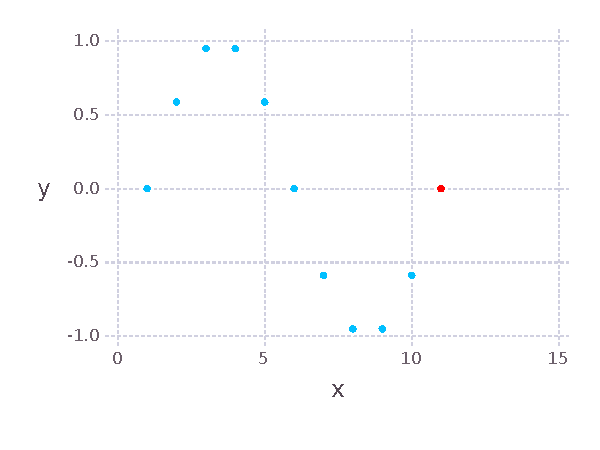
\includegraphics{figures/periodic-data}
\caption{When specifying periodic boundary conditions with \texttt{OnGrid}, the data point on the edge should only be included \emph{once}; the red point should \emph{not} be included in the data.}
\label{fig:periodic-data-spec}
\end{figure}

\paragraph{\texttt{Quadratic\{Periodic,OnCell\}}}
\paragraph{\texttt{Quadratic\{Periodic,OnGrid\}}}
\begin{align*}
\begin{bmatrix}
\frac{3}{4} & \frac{1}{8} & \cdots & & \frac{1}{8}\\
\frac{1}{8} & \frac{3}{4} & \frac{1}{8} \\
 & \frac{1}{8} & \frac{3}{4} & \frac{1}{8} \\
 & & \ddots & \ddots & \ddots
\end{bmatrix}
\begin{bmatrix}c_1\\ c_2\\ c_3\\\vdots\end{bmatrix}
&=
\begin{bmatrix}v_1 \\ v_2 \\ c_3\\\vdots\end{bmatrix}
\end{align*}

Also: $y_1(\delta x) = c_N (\frac{1}{2} - \delta x)^2 + c_1 (\frac{3}{4} - \delta x^2) + c_2(\frac{1}{2} + \delta x)^2$ (note the index on the first coefficient) with a similar wrapping applied at the upper boundary.

\nocite{*}
\printbibliography

\end{document}
